% Presentation for Software Quality Metrics Analysis
\documentclass[aspectratio=169]{beamer}

% Theme and color settings
\usetheme{Madrid}
\usecolortheme{default}

% Packages
\usepackage{graphicx}
\usepackage{booktabs}
\usepackage{tikz}
\usepackage{pgfplots}
\pgfplotsset{compat=1.18}

% Title information
\title{Software Quality Metrics Analysis of Open Source Projects}
\subtitle{A Study of LangChain and Intel XPU Backend for Triton}
\author{Garrett Gruss}
\institute{Southern Methodist University}
\date{\today}

% Remove navigation symbols
\setbeamertemplate{navigation symbols}{}

% Footer with slide numbers
\setbeamertemplate{footline}[frame number]

\begin{document}

% Title slide
\begin{frame}
  \titlepage
\end{frame}

% Outline
\begin{frame}{Outline}
  \tableofcontents
\end{frame}

\section{Introduction}

\begin{frame}{Background}
  \begin{itemize}
    \item Software quality metrics are essential for data-driven decisions in modern development
    \item Internal metrics (complexity, LOC) predict external quality (reliability, maintainability)
    \item DORA metrics have become industry standards for DevOps performance
    \item Open source projects need systematic quality assessment
  \end{itemize}

  \vspace{0.5cm}
  \textbf{Key Challenge:} How do we measure quality in projects we don't control?
\end{frame}

\begin{frame}{Motivation \& Objectives}
  \begin{columns}
    \begin{column}{0.5\textwidth}
      \textbf{Motivation}
      \begin{itemize}
        \item Systematically assess software quality
        \item Identify best practices
        \item Establish reusable benchmarks
        \item Provide actionable insights
      \end{itemize}
    \end{column}

    \begin{column}{0.5\textwidth}
      \textbf{Objectives}
      \begin{itemize}
        \item Collect quality metrics over one month
        \item Analyze project health
        \item Compare across projects
        \item Generate quantitative insights
      \end{itemize}
    \end{column}
  \end{columns}
\end{frame}

\begin{frame}{Selected Projects}
  \begin{columns}
    \begin{column}{0.5\textwidth}
      \textbf{LangChain}
      \begin{itemize}
        \item Framework for LLM applications
        \item Built in Python
        \item 128k stars, 20k forks
        \item 3,812 active contributors
        \item Analysis period: Oct 29 - Nov 27, 2025
      \end{itemize}
    \end{column}

    \begin{column}{0.5\textwidth}
      \textbf{Intel XPU Backend for Triton}
      \begin{itemize}
        \item Compiler backend for Intel GPUs
        \item Out-of-tree Triton module
        \item 222 stars, 78 forks
        \item 538 active contributors
        \item Analysis period: Nov 4 - Dec 2, 2025
      \end{itemize}
    \end{column}
  \end{columns}
\end{frame}

\section{Methodology Evolution}

\begin{frame}{Methodology: Three Phases}
  \begin{center}
    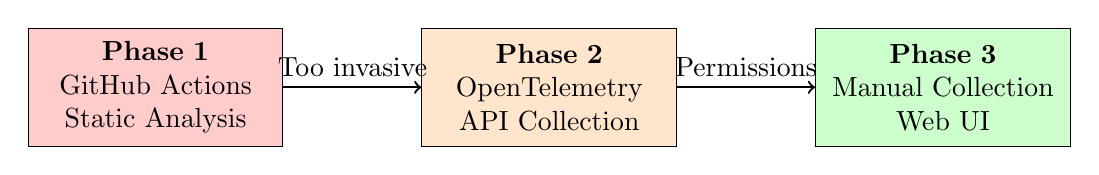
\begin{tikzpicture}[node distance=5cm]
      \node (phase1) [rectangle, draw, fill=red!20, text width=3cm, text centered, minimum height=1.5cm]
        {\textbf{Phase 1}\\ GitHub Actions\\ Static Analysis};
      \node (phase2) [rectangle, draw, fill=orange!20, text width=3cm, text centered, minimum height=1.5cm, right of=phase1]
        {\textbf{Phase 2}\\ OpenTelemetry\\ API Collection};
      \node (phase3) [rectangle, draw, fill=green!20, text width=3cm, text centered, minimum height=1.5cm, right of=phase2]
        {\textbf{Phase 3}\\ Manual Collection\\ Web UI};

      \draw[->, thick] (phase1) -- node[above] {Too invasive} (phase2);
      \draw[->, thick] (phase2) -- node[above] {Permissions} (phase3);
    \end{tikzpicture}
  \end{center}

  \vspace{0.5cm}
  \textbf{Key Lesson:} Methodological flexibility is essential when external constraints arise
\end{frame}

\begin{frame}{Phase 1: GitHub Actions (Abandoned)}
  \begin{columns}
    \begin{column}{0.5\textwidth}
      \textbf{Planned Metrics}
      \begin{itemize}
        \item Lines of Code (LOC)
        \item Cyclomatic Complexity
        \item Code Coverage
        \item Technical Debt
        \item Maintainability Index
      \end{itemize}
    \end{column}

    \begin{column}{0.5\textwidth}
      \textbf{Why Abandoned?}
      \begin{itemize}
        \item Required repository modification
        \item Needed maintainer approval
        \item Risk of workflow conflicts
        \item Per-language customization
        \item \alert{Too invasive for external research}
      \end{itemize}
    \end{column}
  \end{columns}
\end{frame}

\begin{frame}{Phase 2: OpenTelemetry (Blocked)}
  \begin{columns}
    \begin{column}{0.5\textwidth}
      \textbf{Architecture}
      \begin{itemize}
        \item OTel Collector (60s polling)
        \item GitHub GraphQL/REST APIs
        \item OpenObserve storage
        \item Docker Compose deployment
      \end{itemize}

      \vspace{0.3cm}
      \textbf{Target: 9 VCS Metrics}
      \begin{itemize}
        \item vcs.change.count
        \item vcs.change.time\_to\_merge
        \item vcs.ref.lines\_delta
        \item ...and more
      \end{itemize}
    \end{column}

    \begin{column}{0.5\textwidth}
      \begin{figure}
        \centering
        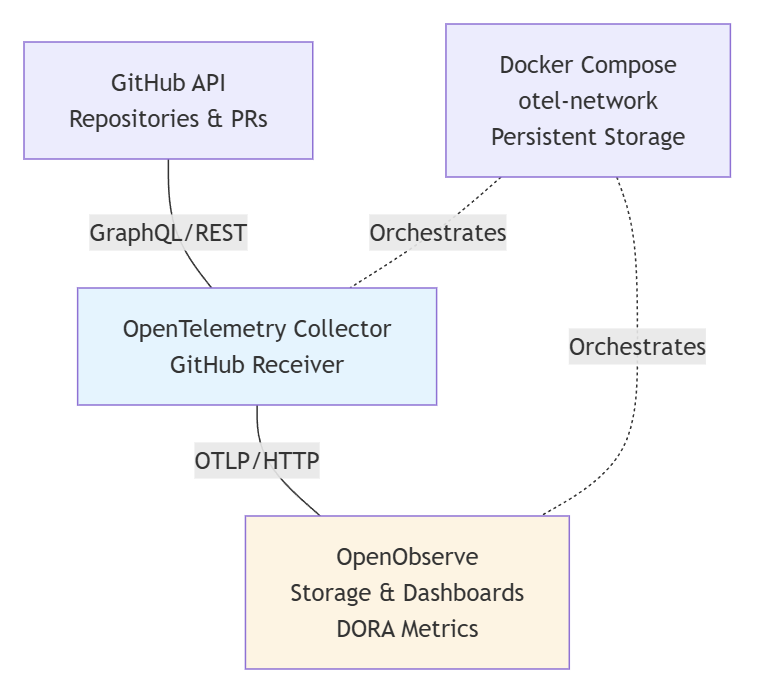
\includegraphics[width=\textwidth]{system-architecture.png}
        \caption{OpenTelemetry Architecture}
      \end{figure}

      \textbf{Blocker:} GitHub PAT requires org admin approval
    \end{column}
  \end{columns}
\end{frame}

\begin{frame}{Phase 3: Manual Collection (Final Approach)}
  \begin{block}{Data Sources}
    \begin{itemize}
      \item GitHub Insights tab (publicly accessible)
      \item Pull Requests page (filtered by date)
      \item Issues page (keyword search)
      \item Organized into CSV format
    \end{itemize}
  \end{block}

  \begin{block}{Advantages}
    \begin{itemize}
      \item No authentication required
      \item No organizational approvals needed
      \item Reproducible by any researcher
      \item Sufficient granularity for DORA metrics
    \end{itemize}
  \end{block}
\end{frame}

\section{DORA Metrics Framework}

\begin{frame}{DORA Metrics: The Four Keys}
  \begin{enumerate}
    \item \textbf{Deployment Frequency (DF)}
    \begin{itemize}
      \item How often code is deployed to production
      \item Proxy: Merged PR rate
    \end{itemize}

    \item \textbf{Lead Time for Changes (LT)}
    \begin{itemize}
      \item Time from commit to production
      \item Measured: PR open-to-merge duration
    \end{itemize}

    \item \textbf{Change Failure Rate (CFR)}
    \begin{itemize}
      \item Percentage of deployments causing failures
      \item Calculated: Bug issues / Total deployments
    \end{itemize}

    \item \textbf{Time to Restore Service (MTTR)}
    \begin{itemize}
      \item Recovery time from failures
      \item Measured: Bug report to fix merge
    \end{itemize}
  \end{enumerate}
\end{frame}

\begin{frame}{DORA Performance Classifications}
  \begin{table}
    \centering
    \small
    \begin{tabular}{@{}lcccc@{}}
      \toprule
      \textbf{Metric} & \textbf{Elite} & \textbf{High} & \textbf{Medium} & \textbf{Low} \\
      \midrule
      Deployment Freq. & Multiple/day & Weekly & Monthly & $<$ Monthly \\
      Lead Time & $<$ 1 day & 1-7 days & 1-4 weeks & $>$ 1 month \\
      Change Failure & 0-15\% & 16-30\% & 31-45\% & $>$ 45\% \\
      Time to Restore & $<$ 1 hour & $<$ 1 day & 1-7 days & $>$ 1 week \\
      \bottomrule
    \end{tabular}
    \caption{2023 DORA State of DevOps Report Classifications}
  \end{table}
\end{frame}

\section{Results}

\begin{frame}{LangChain: Data Overview}
  \textbf{Analysis Period:} October 29 - November 27, 2025 (30 days)

  \vspace{0.5cm}
  \begin{columns}
    \begin{column}{0.5\textwidth}
      \textbf{Pull Requests}
      \begin{itemize}
        \item 179 merged PRs
        \item 67 opened PRs
        \item 89 closed PRs
      \end{itemize}
    \end{column}

    \begin{column}{0.5\textwidth}
      \textbf{Issues}
      \begin{itemize}
        \item 69 total issues
        \item 16 bug-related (23.2\%)
      \end{itemize}
    \end{column}
  \end{columns}
\end{frame}

\begin{frame}{LangChain: Deployment Frequency}
  \begin{columns}
    \begin{column}{0.5\textwidth}
      \textbf{Metrics}
      \begin{itemize}
        \item Mean: 5.97 deployments/day
        \item Median: 8.5 deployments/day
        \item Weekly: 41.77 deployments
        \item Maximum: 46 in one day
      \end{itemize}

      \vspace{0.5cm}
      \begin{block}{Classification: \textcolor{green}{ELITE}}
        Multiple deployments per day indicates mature CI/CD pipeline
      \end{block}
    \end{column}

    \begin{column}{0.5\textwidth}
      \begin{figure}
        \centering
        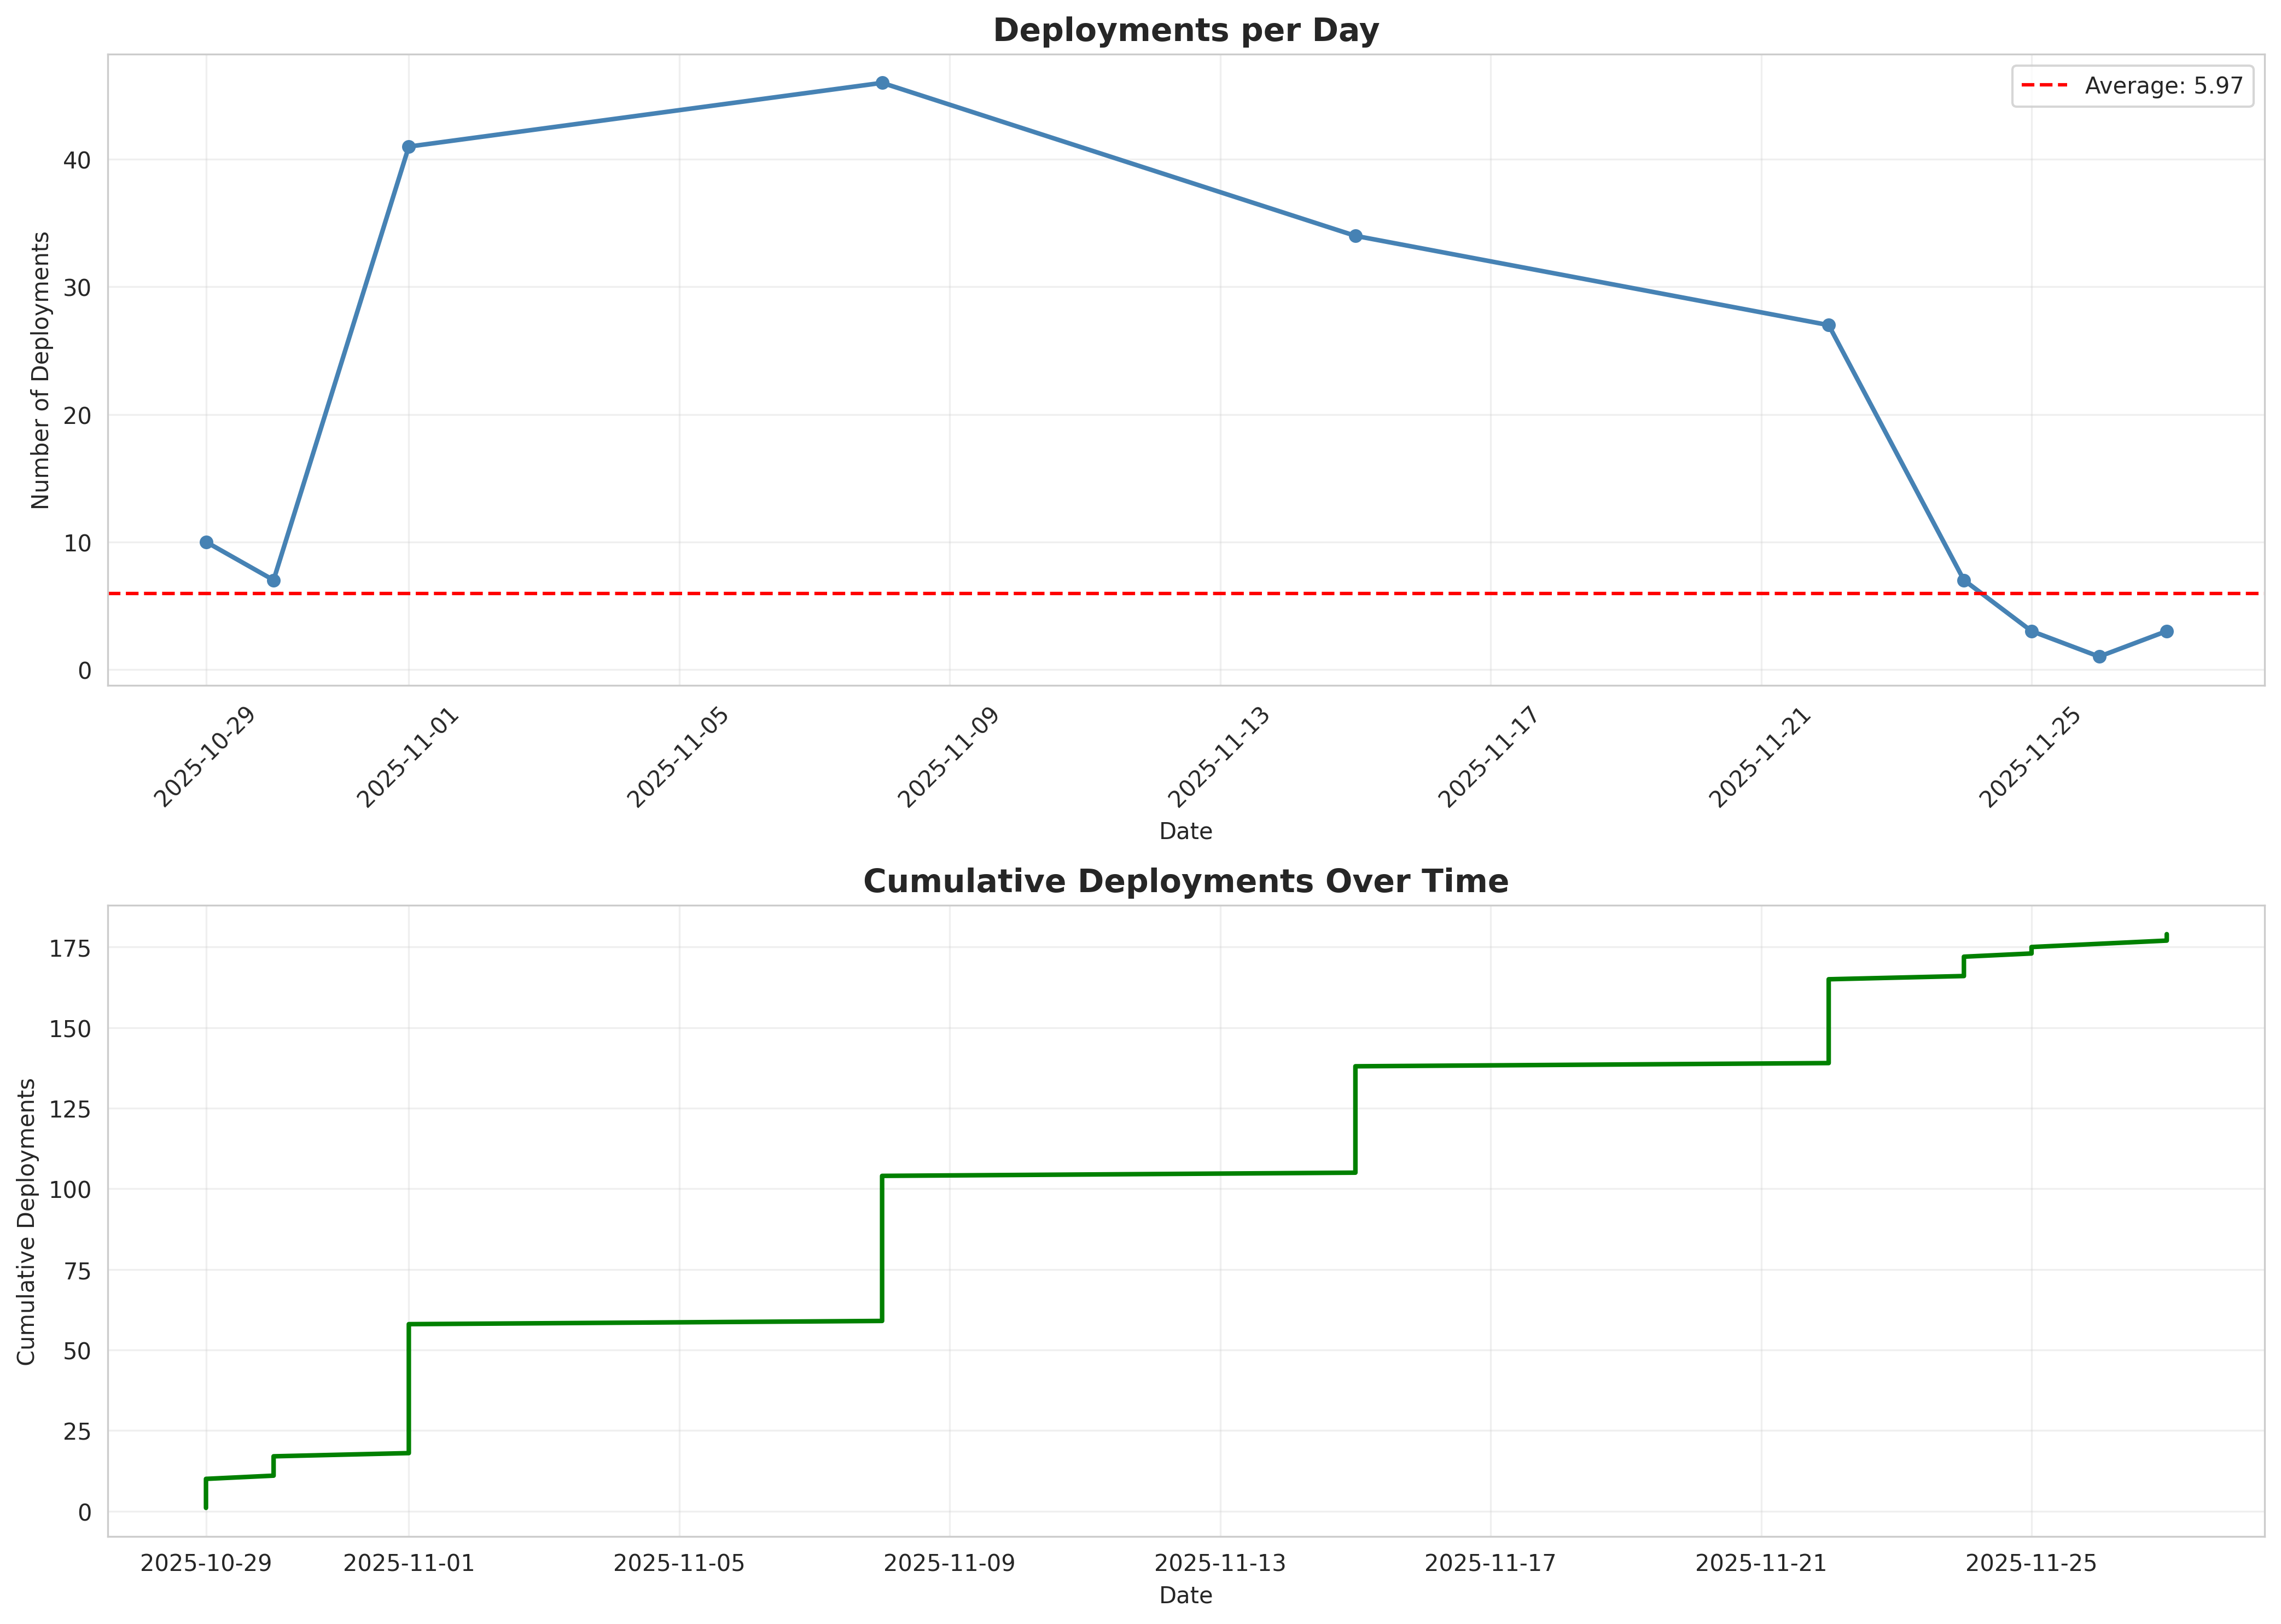
\includegraphics[width=\textwidth]{graphics/langchain_deployment_frequency.png}
      \end{figure}
    \end{column}
  \end{columns}
\end{frame}

\begin{frame}{LangChain: Lead Time \& Change Failure Rate}
  \begin{columns}
    \begin{column}{0.5\textwidth}
      \textbf{Lead Time for Changes}
      \begin{itemize}
        \item Median: 6.00 days
        \item Mean: 4.98 days
        \item 25th percentile: 2.00 days
        \item 90th percentile: 7.00 days
        \item 5 PRs merged within 24 hours
      \end{itemize}

      \begin{block}{Classification: \textcolor{orange}{HIGH}}
        Efficient code review process
      \end{block}
    \end{column}

    \begin{column}{0.5\textwidth}
      \textbf{Change Failure Rate}
      \begin{itemize}
        \item 16 bug issues / 179 deployments
        \item CFR: 8.94\%
        \item Well below 15\% threshold
      \end{itemize}

      \begin{block}{Classification: \textcolor{green}{ELITE}}
        Excellent code quality and testing practices
      \end{block}
    \end{column}
  \end{columns}
\end{frame}

\begin{frame}{LangChain: Summary}
  \begin{table}
    \centering
    \begin{tabular}{@{}lll@{}}
      \toprule
      \textbf{Metric} & \textbf{Value} & \textbf{Classification} \\
      \midrule
      Deployment Frequency & 5.97/day, 41.77/week & \textcolor{green}{Elite} \\
      Lead Time for Changes & 6.00 days (median) & \textcolor{orange}{High} \\
      Change Failure Rate & 8.94\% & \textcolor{green}{Elite} \\
      Time to Restore Service & N/A & N/A \\
      \midrule
      \textbf{Overall Rating} & \multicolumn{2}{l}{\textbf{High Performer}} \\
      \bottomrule
    \end{tabular}
  \end{table}
\end{frame}

\begin{frame}{Intel XPU: Data Overview}
  \textbf{Analysis Period:} November 4 - December 2, 2025 (29 days)

  \vspace{0.5cm}
  \begin{columns}
    \begin{column}{0.5\textwidth}
      \textbf{Pull Requests}
      \begin{itemize}
        \item 104 merged PRs
        \item 17 opened PRs
        \item 73 closed PRs
      \end{itemize}
    \end{column}

    \begin{column}{0.5\textwidth}
      \textbf{Issues}
      \begin{itemize}
        \item 42 total issues
        \item 11 bug-related (26.2\%)
      \end{itemize}
    \end{column}
  \end{columns}
\end{frame}

\begin{frame}{Intel XPU: Deployment Frequency \& Change Failure Rate}
  \begin{columns}
    \begin{column}{0.5\textwidth}
      \textbf{Deployment Frequency}
      \begin{itemize}
        \item Mean: 3.59 deployments/day
        \item Median: 9.0 deployments/day
        \item Weekly: 25.10 deployments
        \item Maximum: 28 in one day
      \end{itemize}

      \begin{block}{Classification: \textcolor{green}{ELITE}}
        Multiple deployments per day for compiler backend
      \end{block}
    \end{column}

    \begin{column}{0.5\textwidth}
      \textbf{Change Failure Rate}
      \begin{itemize}
        \item 11 bug issues / 104 deployments
        \item CFR: 10.58\%
        \item Below 15\% threshold
      \end{itemize}

      \begin{block}{Classification: \textcolor{green}{ELITE}}
        Strong quality controls for complex domain
      \end{block}
    \end{column}
  \end{columns}
\end{frame}

\begin{frame}{Intel XPU: Summary}
  \begin{table}
    \centering
    \begin{tabular}{@{}lll@{}}
      \toprule
      \textbf{Metric} & \textbf{Value} & \textbf{Classification} \\
      \midrule
      Deployment Frequency & 3.59/day, 25.10/week & \textcolor{green}{Elite} \\
      Lead Time for Changes & N/A (insufficient data) & N/A \\
      Change Failure Rate & 10.58\% & \textcolor{green}{Elite} \\
      Time to Restore Service & N/A & N/A \\
      \midrule
      \textbf{Overall Rating} & \multicolumn{2}{l}{\textbf{Elite Performer*}} \\
      \bottomrule
    \end{tabular}
  \end{table}

  \vspace{0.3cm}
  \small{* Based on elite performance in deployment frequency and change failure rate}
\end{frame}

\begin{frame}{Comparative Analysis}
  \begin{table}
    \centering
    \begin{tabular}{@{}lll@{}}
      \toprule
      \textbf{Metric} & \textbf{LangChain} & \textbf{Intel XPU} \\
      \midrule
      Deployment Frequency & 5.97/day (Elite) & 3.59/day (Elite) \\
      Lead Time for Changes & 6.00 days (High) & N/A \\
      Change Failure Rate & 8.94\% (Elite) & 10.58\% (Elite) \\
      Time to Restore Service & N/A & N/A \\
      \midrule
      Overall Rating & High Performer & Elite Performer \\
      \bottomrule
    \end{tabular}
  \end{table}

  \vspace{0.3cm}
  \textbf{Key Insights:}
  \begin{itemize}
    \item Both projects show elite deployment frequency
    \item Both maintain excellent change failure rates (<15\%)
    \item LangChain has measurable lead time in high performance range
  \end{itemize}
\end{frame}

\section{Discussion}

\begin{frame}{Key Findings}
  \begin{block}{Development Velocity}
    Both projects demonstrate elite-level deployment frequency, indicating mature CI/CD pipelines and rapid iteration capabilities
  \end{block}

  \begin{block}{Code Quality}
    Change failure rates below 15\% suggest:
    \begin{itemize}
      \item Comprehensive test coverage
      \item Effective code review processes
      \item Strong quality gates
    \end{itemize}
  \end{block}

  \begin{block}{Data Limitations}
    \begin{itemize}
      \item MTTR could not be calculated (no bug-fix pair linking)
      \item Intel XPU had insufficient lead time data (only 3 matched PRs)
      \item One-month window may not capture long-term trends
    \end{itemize}
  \end{block}
\end{frame}

\begin{frame}{Lessons Learned: Technical Challenges}
  \begin{enumerate}
    \item \textbf{Repository Access Tradeoffs}
    \begin{itemize}
      \item Internal metrics require invasive modifications
      \item External research needs non-invasive approaches
    \end{itemize}

    \item \textbf{API \& Permission Constraints}
    \begin{itemize}
      \item GitHub PAT requires organizational approval
      \item Rate limits (5,000/hr auth, 60/hr unauth)
      \item Broad permission scopes create gatekeeping
    \end{itemize}

    \item \textbf{Data Completeness vs. Accessibility}
    \begin{itemize}
      \item Phase 1: Max richness, max invasiveness
      \item Phase 2: Moderate richness, still blocked
      \item Phase 3: Min richness, universal access
    \end{itemize}
  \end{enumerate}
\end{frame}

\begin{frame}{Lessons Learned: Best Practices}
  \textbf{Best Practices for External Software Quality Research:}

  \begin{enumerate}
    \item Start with minimal access assumptions
    \item Prioritize non-invasive observation
    \item Leverage public observability (GitHub Insights)
    \item Use industry-standard frameworks (DORA, SPACE)
    \item Automate analysis, not collection
    \item Build incremental validation
    \item Document methodological pivots
  \end{enumerate}

  \vspace{0.5cm}
  \textbf{Value of DORA Metrics:}
  \begin{itemize}
    \item Industry standardization enables benchmarking
    \item Publicly derivable from GitHub data
    \item Actionable elite/high/medium/low classifications
  \end{itemize}
\end{frame}

\section{Conclusion}

\begin{frame}{Future Work}
  \begin{columns}
    \begin{column}{0.5\textwidth}
      \textbf{Extended Data Collection}
      \begin{itemize}
        \item 3-6 month analysis periods
        \item Additional open source projects
        \item Longitudinal trend analysis
      \end{itemize}

      \vspace{0.3cm}
      \textbf{Enhanced Metrics}
      \begin{itemize}
        \item Code-level metrics (if access obtained)
        \item Contributor activity patterns
        \item Code review analytics
      \end{itemize}
    \end{column}

    \begin{column}{0.5\textwidth}
      \textbf{ML Applications}
      \begin{itemize}
        \item Predict project health from trends
        \item NLP for better issue classification
        \item Anomaly detection in dev patterns
      \end{itemize}

      \vspace{0.3cm}
      \textbf{Tool Development}
      \begin{itemize}
        \item Real-time DORA dashboard
        \item SaaS for OSS health analysis
        \item CI/CD pipeline integration
      \end{itemize}
    \end{column}
  \end{columns}
\end{frame}

\begin{frame}{Conclusion}
  \begin{block}{Summary}
    This study successfully analyzed software quality metrics for LangChain and Intel XPU Backend for Triton using DORA metrics derived from publicly accessible GitHub data.
  \end{block}

  \begin{block}{Key Achievements}
    \begin{itemize}
      \item Demonstrated adaptive methodology in face of technical constraints
      \item Validated DORA metrics as effective quality indicators
      \item Established reproducible approach for external research
      \item Provided actionable insights into project health
    \end{itemize}
  \end{block}

  \begin{block}{Impact}
    The methodology developed is reproducible and can be applied to any open source project with public GitHub repositories, enabling systematic quality assessment without requiring repository access.
  \end{block}
\end{frame}

\begin{frame}[plain,standout]
  \centering
  \Huge Questions?

  \vspace{1cm}
  \normalsize
  Garrett Gruss \\
  Southern Methodist University

  \vspace{0.5cm}
  \small
  Software Quality Metrics Analysis of Open Source Projects
\end{frame}

\end{document}
